\documentclass{article}

\usepackage[german]{babel}
\usepackage[utf8]{inputenc}

\usepackage{amsfonts}
\usepackage{amssymb}
\usepackage{amsmath}

\usepackage{color}

\usepackage{graphicx}
\usepackage{hyperref}

\usepackage{multicol}

\usepackage[top=1cm, left=1cm, right=1cm, bottom=1cm, a4paper]{geometry}

% Platzsparende Überschriften
\newcommand{\h}[1]{\vspace{1ex}\begin{center}\small\textbf{#1}\end{center}}
\newcommand{\hh}[1]{{\vspace{1pt}\hrule\vspace{1pt} \noindent\textbf{#1}}\\}
\newcommand{\hhh}[1]{{\vspace{1pt}\noindent\emph{#1:}}}
\setlength{\parindent}{2ex}

\newenvironment{tightlist}{
\begin{list}{\textbullet}{
\setlength{\topsep}{-1ex}
\setlength{\itemsep}{-1ex}
\setlength{\leftmargin}{4ex}
}
}{
\end{list}
\vspace{1ex}
}

\newcounter{Lcount}
\newenvironment{tightenum}{
\begin{list}{\arabic{Lcount}.}{
\usecounter{Lcount}
\setlength{\topsep}{-1ex}
\setlength{\itemsep}{-1ex}
\setlength{\leftmargin}{4ex}}
}{
\end{list}
\vspace{1ex}
}

% FIXME
\newcommand{\FM}[1]{{\color{red}\emph{#1}}}

\setlength{\topsep}{0ex}

\pagestyle{empty}
\begin{document}
\begin{center} 1 Din A4 Zettel mit beliebigem Inhalt\end{center}

\begin{multicols}{4}
\scriptsize\raggedright

\setlength{\parskip}{0pt}

\h{Entscheidbarkeit}
\hh{Nichtentscheidbare Probleme}
\FM{Welche von denen gehören zu den Semientscheidbaren?}
\begin{tightlist}
\item Diagonalsprache
	$L_d:=\{\omega_i: M_i$ akzeptiert $\omega_i$ nicht$\}$
\item Kontextfreie Sprachen:
$L(G_1) \subseteq L(G_2)$?,
Mehrdeutigkeit (mehrere Ableitungen zum gleichen Wort)?,
$\overline{L(G)}$ kontextfrei?,
$L(G)$ regulär?,
$L(G)$ det. kontextfrei?
\item Diophantische Gleichungen: multivariates Polynome $p$, Koeffizienten ganzzahlig: $\exists x_1, \ldots, x_n\in\mathbb{Z}:p(x_1, \ldots, x_n)=0$?
\item \emph{siehe semientsch. Probleme}
\end{tightlist}


\hh{Semientscheidbare Probleme}
\hhh{Definition} Es ex. eine TM, die genau die Wörter aus $L$ akzeptiert, sonst aber nicht halten muss.

\hhh{Beispiele}
\begin{tightlist}
\item Halteproblem 
	$H:=\{wv | T_w$ hält auf der Eingabe $v\}$
\item Universelle Sprache
	$L_u:=\{wv| v\in L(T_w)\}$
\item Postsches Korrenspondenzproblem\ Geg: Menge von Wortpaaren $(x_i , y_i) \in (\Sigma^+ \times \Sigma^+)^*$.\ Gibt es eine endl. Folge von Indizes: $x_{i1} ... x_{in}=y_{i1}... y_{in}$?
\item Komplement der Diagonalsprache
\end{tightlist}

% \hhh{\FM{Chomsky-Hierarchie}}

\hh{Entscheidbare Probleme}
\hhh{Definition} Es ex. eine TM, die genau die Wörter aus $L$ akzeptiert und bei jeder Eingabe hält.
\hhh{Beispiele}\\
\hhh{Presburger Arithmetik} eingeschränkte prädikatenlogische Formeln.\\
\begin{tabular}{l|c|c|c|c}
Typ & $\in$ & $\emptyset$ & $=$ &$\cap=\emptyset$ \\
\hline
CH-3 & J & J & J & J \\
Det. KF & J & J & J & N \\
CH-2& J & J & N & N \\
CH-1& J & N & N & N \\
CH-0& N & N & N & N  
\end{tabular}


\h{$\mathcal{NP} \stackrel{?}= \mathcal{P}$}
\hh{Definitionen $\mathcal{NP}, \mathcal{P}$ }
\begin{tightlist}
\item {time$_M(w)$} $:=$ Anzahl Rechenschritte einer TM $M$ bei Eingabe $w$\\
\item {TIME$(f(n))$} $:=\{L\in\Sigma^*:\exists$ TM $M:L(M) = L$ und $\forall w\in L(M):$ time$_M(w)\le f(|w|)\}$\\
\item {$\mathcal{P}$} $:=\cup_{\text{Polynom }p}\text{TIME}(p(n) )$\\
\item {ntime$_M(w)$} $=\begin{cases}\text{min}\{n:P=(s)w\Rightarrow^n u(f)v,\\ f\in F\} \text{ falls }w\in L(M)\\ 0,\ \text{sonst}\end{cases}$\\
\item {NTIME$(f(n))$} $=\{L\in\Sigma^*:\exists\text{NTM}\ M:L(M) = L\text{ und }\forall w\in L(M):\text{ntime}_M(w)\le f(|w|)\}$\\
\item {$\mathcal{NP}$} $=\cup_{\text{Polynom }p}\text{NTIME}(p(n))$\\
\item $V\in\mathcal{NP}$-hart $:\Leftrightarrow$ $\forall V'\in\mathcal{NP}: V'\le_pV$
\item $V\in\mathcal{NP}$-vollständig $:\Leftrightarrow$ $V\in \mathcal{NP}\cap\mathcal{NP}$-hart
\end{tightlist}

\emph{Probleme siehe Tabelle}
Achtung: "`Rucksack"' ist Knapsack bei Sanders, aber Subsetsum bei Schöning.

\h{Grammatiken}
Sei $G=(V, \Sigma, P, S)$, $\forall l\to r\in P:$\\
\hh{Def. CH-0 (rekursiv aufzählbar)}
beliebig\\
\hhh{Wortproblemkomplexität} semientscheidbar
\hh{Definition CH-1 (längenbeschr.)}
$|l|\le |r|$. Sonderregel für $\varepsilon$-Produktion nur bei $S$\\
\hhh{Beispiel} $a^nb^nc^n$\\
\hhh{Wortproblemkomplexität}\\ $|\Sigma|^{O(n)}$, NP-hart
\hhh{Entscheidbare Probleme}
$L(G) = \emptyset$, $|L(G)|\ne\infty$, $L(G)=\Sigma^*$

\hh{Definition CH-2 (kontextfrei)}
CH-1 und $l\in V$\\
\hhh{Beispiel} $a^nb^n$\\
\hhh{Wortproblemkomplexität} $O(n^3)$
\hhh{Pumpinglemma}
$L$ kontextfrei $\Rightarrow\exists n\in\mathbb{N}:\forall z\in L, |z|> n: \exists u, v, w, x, y:$\\$z=uvwxy\wedge|vx|\ge 1\wedge|vwx|\le n \wedge \forall i\in \mathbb{N}_0:uv^iwx^iy\in L$\\
\hhh{Odgens Lemma} 
$L$ kontextfrei $\Rightarrow\exists n\in\mathbb{N}:\forall z\in L, |z|\ge n:$ Wenn wir in $z$ mindestens $n$ Buchstaben markieren $\exists u, v, w, x, y: z = uvwxy$, dass von den mindestens $n$ markierten Buchstaben mindestens einer zu $vx$ gehört und höchstens $n$ zu $vwx$ gehören und $\forall i \ge 0: uv^iwx^iy \in L$.\\
\hhh{Chomsky-Normalform}
falls gilt: $P\subseteq (V\times\Sigma)\cup( V\times VV)$
\begin{tightenum}
\item Terminale in eigene Regeln.
\item Regeln mit rechts $>2$ Nicht-Terminale aufsplitten
\item $\varepsilon$-Produktionen entfernen
\item Kettenproduktionen entfernen
\end{tightenum}

\hh{Definition Det. KF}
\FM{Bitte noch eintragen}
\hhh{Wortproblemkomplexität} $O(n)$

\hh{Definition CH-3 (regulär)}
CH-2 und $r\in\Sigma\cup\Sigma V$\\
\hhh{Beispiel} $a^*b^*$\\
\hhh{Wortproblemkomplexität} $O(n)$
\hhh{Pumpinglemma}
$L$ regulär $\Rightarrow\exists n\in\mathbb{N}:\forall w\in L,|w|> n: \exists u, v, x:w=uvx\wedge|v|\ge 1\wedge|uv|\le n\wedge\forall i\in\mathbb{N}_0:uv^ix\in L$\\
\hhh{Reguläre Ausdrücke}\\
Beispiel: $(\emptyset\cup\varepsilon)^*abc^+$\\
%noch mehr als Beispielausdruck?

\hh{Nerode-Relation}
\hhh{Für Sprache $L$}
$R_L:=\{(x, y)\in \Sigma^*\times\Sigma^*:\forall z\in\Sigma^*:xz\in L\Leftrightarrow yz\in L\}$\\
\hhh{Für Automat $M$}
$R_M:=\{(x, y)\in \Sigma^*\times\Sigma^*:\delta^*(s,x) = \delta^*(s,y)\}$ \\
\hhh{Verfeinerung} $R$ verfeinert $R'\Leftrightarrow R\subseteq R'$\\
\hhh{Satz}
$L$ regulär $\Leftrightarrow$ index$(R_L)\ne\infty$\\
\hhh{Satz}
$q \not\equiv r\Leftrightarrow\exists z\in\Sigma^*:\delta(q, z)\in F\not\Leftrightarrow\delta(r, z)\in F$\\
\hhh{Beispielanwendung}
$a^nb^n$ ist nicht regulär, denn $[a^n],n\in\mathbb{N}$ sind unendlich verschiede Äquivalenzklassen, denn für $i\ne j$ ist $a^ib^i\in L$, aber $a^jb^i\notin L$, also $[a^i] \ne [a^j]$.

\hh{Abschlusseigenschaften}
\begin{tabular}{l|c|c|c|c|c}
Typ & $\cap$ & $\cup$ & $\overline{\color{white}L}$ & $\cdot$ & $*$\\
\hline
CH-3 & J & J & J & J & J \\
Det. KF & N & N & J & N & N \\
CH-2& N & J & N & J & J \\
CH-1& J & J & J & J & J \\
CH-0& J & J & N & J & J \\
semient. & J & J & N & J & J \\
entsch.  & J & J & J & J & J
\end{tabular}
%\FM{bei semient. und ent. stand "`N"' bei $\cdot$ und $*$, ich glaub "`J"'. weiß jemand mehr?}

\hh{Automaten-Zuordnung}


\begin{tabular}{r|l}
Typ  & Automat \\
\hline
CH-3 & Endlicher Automat \\
     & (NEA, DEA) \\
Det. KF & det. Kellerautomat\\
        & (DKellerA) \\
CH-2 & Kellerautomat \\ 
     & (NKellerA) \\
CH-1 & linear beschr. Automat\\
     & (NLBTM) \\ % War das nicht ne ISDN-Anschlusdose?
CH-0 & Turingmaschine (TM) 
\end{tabular}

\hh{Automatenäquivalenz}
$\varepsilon$NEA ist zu $\overline\varepsilon$NEA ist zu DEA und NTM ist zur DTM äquivalent. NKellerA ist zu DKellerA nicht äquivalent. Äquivalenz von NLBTM und DLBTM ist noch nicht bewiesen.

\h{Automaten}

Mealy-Automat: Ausgabe beim Übergang, Moore-Automat: Ausgabe beim Zustand.
\hh{DTM}
$T=(Q, \Sigma, \Gamma, \delta, s, F ), \delta: Q\times\Gamma\to Q\times\Gamma\times\{L, R, N\}$\\
\hhh{sie hält in $q(q)av$} $\Leftrightarrow\delta(q, a)=(q,a,N).$\\
Konvention: $\forall q\in F:\forall a\in\Gamma:\delta(q, a) = (q, a, N)$\\
\hhh{sie akzeptiert $w$} $\Leftrightarrow (s)w$ hält nach endlich vielen Übergängen in $x(f)y, f\in F$. $y$ ist die Ausgabe.\\
\hhh{rekursiv aufzählbar (semientscheidbar)} $\exists T:T$ akzeptiert $L$\\
\hhh{rekursiv (entscheidbar)} $\exists T: T$ akzeptiert $L\wedge\forall w\in\Sigma^*:T$ hält.\\

\hh{DTM-Varianten}
Mehrere Bänder, mehrere Köpfe, mehrere Dimensionen -- alles gleich mächtig wie DTM.

\hh{NTM}
$T=(Q, \Sigma, \Gamma, \delta, s, F ), \delta: Q\times\Gamma\to 2^{Q\times\Gamma\times\{L, R, N\}}$\\
\hhh{sie hält wie} DTM\\
\hhh{sie akzeptiert $w$}$\Leftrightarrow\exists$ Folge von Konfigurationen $s(w)\to\cdots\to x(f)y, f\in F$\\ 

\hh{Gödelnummer-Code}
1. Kodiere $\delta$: \\
$\delta(q_i,a_j)=(q_r,a_s,d_t) \to 0^i10^j10^r10^s10^t$ \\
wobei $d_t\in \{d_1=L, d_2=R, d_3=N\}$ \\
2. Die TM wird dann kodiert durch: \\
			$111u_1 11u_211...11u_z111$ \\
			mit $u_i$ die möglichen Übergänge in bel. Reihenfolge. \\

\hh{NLBTM}
NTM $T=(Q, \Sigma, \Gamma, \delta, s, F): \forall a=a_1,\ldots, a_n\in\Sigma^+:a\stackrel{*}{\Rightarrow}\alpha(q)\beta$ mit $|\alpha\beta|<n$

\hh{Nichtdet. Kellerautomat}
$K=(Q, \Sigma, \Gamma, \delta, s, \#), \delta: Q\times(\Sigma\cup\varepsilon)\times\Gamma\to 2^{Q\times\Gamma^*}$\\
\hhh{er akzeptiert $w$} $\Leftrightarrow\exists$ Folge von Konfigurationen $(s, w, \#)\to\cdots\to(q, \varepsilon, \varepsilon), q\in Q$ beliebig.\\
\hh{Det. Kellerautomat}
$K=(Q, \Sigma, \Gamma, \delta, s, \#), \delta: Q\times(\Sigma\cup\varepsilon)\times\Gamma\to 2^{Q\times\Gamma^*}$ mit $\forall q\in Q, a\in\Sigma, A\in\Gamma:|\delta(z, a, A)|+|\delta(z, \varepsilon, A)|\le 1$\\
\hhh{er akzeptiert $w$} $\Leftrightarrow\exists$ Folge von Konfigurationen $(s, w, \#)\to\cdots\to(f, \varepsilon, \varepsilon), f\in F$\\
\hh{Automatenminimierung}
(Für endliche Automaten)
\begin{tightenum}
\item nicht erreichbare Zustände weg \\
\item Tabelle aller Zustandspaare $\{z,z'\}$ mit $z \neq z'$ \\
($z_1$ bis $z_k$ links, $z_0$ bis $z_{k-1}$ unten) \\
\item Markieren der Zustandspaare mit $z \in F$ und $z \notin F$ oder umgekehrt. \\
\item Betrachte unmakrierte Paare $\{z,z'\}$. \\
Wenn $\{\delta(z,a),\delta(z',a)\}$ für mind. ein $a \in \Sigma$ bereits makiert, markiere $\{z,z'\}$. \\
\item Wiederhole 4. bis keine Änderung mehr. \\
\item Unmarkierte Paare können verschmolzen werden. \\ 
\end{tightenum}

\hh{DEA$\to$reg. ex.}

Betrachte $L_{ij}^m := \{w:\Sigma^*:\text{ Beim Verarbeiten von $w$ geht $A$}$\\$\text{ vom Zustand $i$ nach $j$ und dabei}$\\$\text{ höchstens durch $m$}\}$.\\
Es gilt $L_{ij}^{m+1} = L_{ij}\cup\left( L_{i,m+1}^m (L_{m+1,m+1,}^m)^* L_{m+1,j}^m\right)$\\
So weitermachen, bis man $L_{sf}^n$ hat ($s$ Startzustand, $f$ Endzustand, $n$ Zahl der Zustände).

\hh{NEA $\to$ DEA}
Potenzmengenkonstruktion. Knotenmengen sind Endzustände, wenn einer ihrer enthaltenen Zustände ein Endzustand ist.


%noch andere Maschinenmodelle?
\h{Whileprogramm}
$\mathbb{N}$ main$(\mathbb{N} x_1, \ldots, x_k ) \{$\\
\ $\mathbb{N} x_0 = 0;\mathbb{N} x_{k+1}=0;\ldots$\\
\ body$;$\\
\ return $x_0;$\\
$\}$\\
body $\in\{ $ Sequenz '$;$'$,$while$(x_i\ne 0):$ Schleife$, x_i:=x_i+c$ wobei $c\in\{-1, 0, 1\}$ und $0-1:=0\}$\\
"`loop"'-Konstrukte im body erlaubt, aber redundant.
\h{Loopprogramm}
$\mathbb{N}$ main$(\mathbb{N} x_1, \ldots, x_k ) \{$\\
\ $\mathbb{N} x_0 = 0;\mathbb{N} x_{k+1}=0;\ldots$\\
\ body$;$\\
\ return $x_0;$\\
$\}$\\
body $\in\{ $ Sequenz '$;$'$,$loop$(x_i):$ Schleife, wobei schon vor dem Durchlauf bekannt ist wie oft die Schleife wiederholt wird$, x_i:=x_i+c$ wobei $c\in\{-1, 0, 1\}$ und $0-1:=0\}$\\


\h{Ackermannfunktion}
\hh{Definition}
Function $a(x, y)$\\
if $x=0$ then return $y+1$\\
if $y=0$ then return $a(x-1, 1)$\\
return $a(x-1, a(x, y-1))$\\
\hh{Eigenschaften}
\begin{tightlist}
\item $\forall$ Loopprogramm $P:\exists k:\forall n\in\mathbb{N}:f_P(n)<a(k, n)$
\item $y<a(x, y)$
\item $a(x, y)<a(x, y+1)$
\item $a(x, y+1)<a(x+1, y)$
\item $a(x, y)<a(x+1, y)$
\item $a(x, y)\le a(x', y')$ falls $x\le x'$ und $y\le y'$
\end{tightlist}

\h{Pseudopolinomialität}
Nur relevant für Probleme mit Zahlen
\h{Approximation}
$\mathcal{A}$ ein polynomieller Approximationsalgo, $\text{OPT}$ Optimalwert:\\
\hh{absoluter Approxalgo} $\forall I$ Instanzen eines Optimierungsproblems $\exists K: \text{OPT}(I) - \mathcal{A}(I) \le K$\\
\hh{Approxalgo relativer Güte} $\forall I\text{Instanz}\exists K: \mathcal{R}_{\mathcal{A}}(I)\le K, K\ge 1$ konstant.\\
$\mathcal{R}_{\mathcal{A}}=\begin{cases}\frac{\mathcal{A}(I)}{\text{OPT}(I)}\text{falls Minimierungspr.}\\ \frac{\text{OPT}(I)}{\mathcal{A}(I)}\text{falls Maximierungspr.}\end{cases}$\\
\FM{vll Formulierungen anpassen}\\
\hh{PAS -- Approxschema} Familie von Approxalgos $\mathcal{A}_{\varepsilon}$ mit $\mathcal{R}_{\mathcal{A}_{\varepsilon}}\le 1+\varepsilon$, polynomiell in der Eingabe\\
\hh{FPAS -- vollpoly Approxschema} wie PAS, aber auch polynomiell in $\frac{1}{\varepsilon}$\\

\hh{Ansatz Nichtexistenzbeweis} Man zeigt, dass man das eigentliche Problem aufblähen kann, so dass eine Approximation des aufgeblähten beim zurücktransformieren das eigentliche Problem (in $\mathcal{P}$) lösen würde.

\hh{Bekannte Existenzen}
(Falls $\mathcal{NP}\ne\mathcal{P}$)
\begin{tightlist}
\item KNAPSACK, Clique kein abs. Approx-Algo
\item Knapsack hat rel. Approx-Algo (greedy, Güte 2)
\item Color hat kein rel. Approx-Algo mit $\mathcal{R}^\infty \le \frac43$
\item TSP mit $\Delta$-Ungleichung hat rel. Approx-Algo mit $\mathcal{R}\le 2$
\end{tightlist}

\h{Hinweise}
\FM{Diese Hinweise müssen noch ein sortiert und ggf. umformuliert werden}

% Wie krieg ich diese verdammte einrückung weg?
\begin{tightlist}
\item Bei Reduktionsbeweisen stets zeigen, dass eine Lösung des einen Problems eine Lösung im anderen Problem induziert \textbf{und umgekehrt}. (Dieses muss allerdings nur in der einen Richtung in polynomieller Zeit möglich sein)
\end{tightlist}

\end{multicols}



\pagebreak
\scriptsize\raggedright
\h{NP-Vollständige Probleme}\
		\begin{tabular}{p{1.6cm}p{6cm}p{6cm}p{1.8cm}}
		Problem 		&		Gegeben		&		Gesucht		& polyn. red. von \\ \hline
		SAT					& aussagenlog. Formel & Erfüllbarkeit & TM\\
		3SAT				& boolesche Formel in KNF mit 3 Lit. pro Klausel & Erfüllbarkeit & SAT \\
		Set Cover		& endl. Menge $M$ und $T_1,...,T_k \subseteq M$, Zahl $n \leq k$	&  $n$ Mengen $T_{i_1},...,T_{i_n}$ mit $M=\cup_{j=1\ldots n}T_{i_j}$ & 3SAT \\
		Steiner-Tree& Unger.	Graph $G=(V,E)$ mit Gewichten $c:E \rightarrow \mathbb{R}^+$, $V=R$ (Pflicht-) $\cup$ $F$ (Steinerknoten)	&	Baum $T \subseteq E$ der mit minimalen Kosten alle Pflichtknoten verbindet& 3SAT \\
		Clique			&	ungerichteter Graph $G=(V,E)$ und Zahl $k \in \mathbb{N}$ & Clique $V'\subseteq V$ mit $|V'|\ge k$, also $\forall i,j \in V', i \neq j$, gilt: $\{i,j\} \in E$ & 3SAT \\
		Vertex Cover&	ungerichteter Graph $G=(V,E)$ und Zahl $k \in \mathbb{N}$ &	überdeckende Knotenmenge $V'\subseteq V$ mit $\left| V' \right| \geq k$, sodass $\forall \{u,v\} \in E$: $u \in V'$ oder $v \in V'$	& Clique \\
		Subset Sum & Zahlen $a_1,...,a_k \in \mathbb{N}$ und $W \in \mathbb{N}$ &	Teilmenge $J \subseteq \{1,...,k \}$ mit $\sum_{i \in J}{a_i}=W$ & 3SAT \\ 
		Partition		&	Zahlen $a_1,...,a_k \in \mathbb{N}$ &	Teilmenge $J \subseteq \{1,...,k \}$ mit $\sum_{i \in J}{a_i}=\sum_{i \notin J}{a_i}$	& Subset Sum \\
		Bin Packing &	Behältergröße b $\in \mathbb{N}$, Behälteranzahl k $\in \mathbb{N}$, Objekte $a_1,...a_k \leq b$ & Abb. $f: \{1,...,n\}\rightarrow \{1,...,k\}$, sodass $\forall j=1,..,k: \sum_{f(i)=j}{a_i \leq b}$	& Partition \\
		Knapsack		&	endl. Menge $M$, Gewichsfkt. $w:M \rightarrow \mathbb{N}_0$, Kostenfkt. (Profitfkt.) $c:M \rightarrow \mathbb{N}_0$, $W,C \in \mathbb{N}_0$ & $M' \subseteq M$ mit $\sum_{a \in M'}{w(a)} \leq W$ und $\sum_{a \in M'}{c(a)} \geq C$ & Subset Sum \\
		ILP					&	Vektor $x=(x_1,\ldots,x_n)$ und Bedingungen $a\cdot x R b$ mit $R\in\{\le,\ge,=\}$, $a\in\mathbb{Z}^n$, $b\in\mathbb{Z}$   & Gibt es eine Belegung von $x$, so dass alle Bedingungen erfüllt sind?	& Subset Sum \\
		Gericht. Hamiltonkreis &	gerichteter Graph $G=(V,E)$	&	Hamiltonkreis: einfacher Kreis der jeden Knoten genau einmal enthält	& 3SAT \\
		Hamiltonkreis & ungerichteter Graph $G=(V,E)$	&	Hamiltonkreis	& Gericht. Hamiltonkreis \\
		TSP					& Vollständiger Graph $G=(V,V\times V)$ mit Abstandsfkt. $d:V\times V\to\mathbb{R}^+$ und Zahl $k$ & Hamiltonkreis $C$ mit Länge $\sum_{(u,v)\in C} d(u,v)\le k$ & Hamiltonkreis \\
		Coloring		&	ungerichteter Graph $G=(V,E)$ und Zahl $k \in \mathbb{N}$ &	$c:V\to 1,\ldots,k$ mit $\forall{\{u,v\}\in E}: c(u) \ne c(v)$	& 3SAT \\
								
		\end{tabular}

\begin{center}
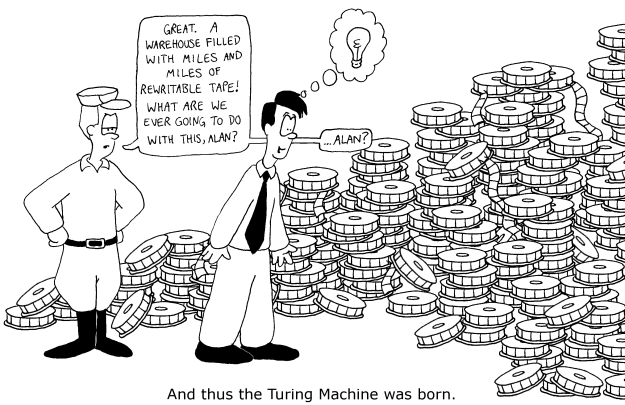
\includegraphics[width=.5\textwidth]{turing.png}
\end{center}

\h{Und für die, die den Taschenrechner vergessen haben:}
\begin{center}
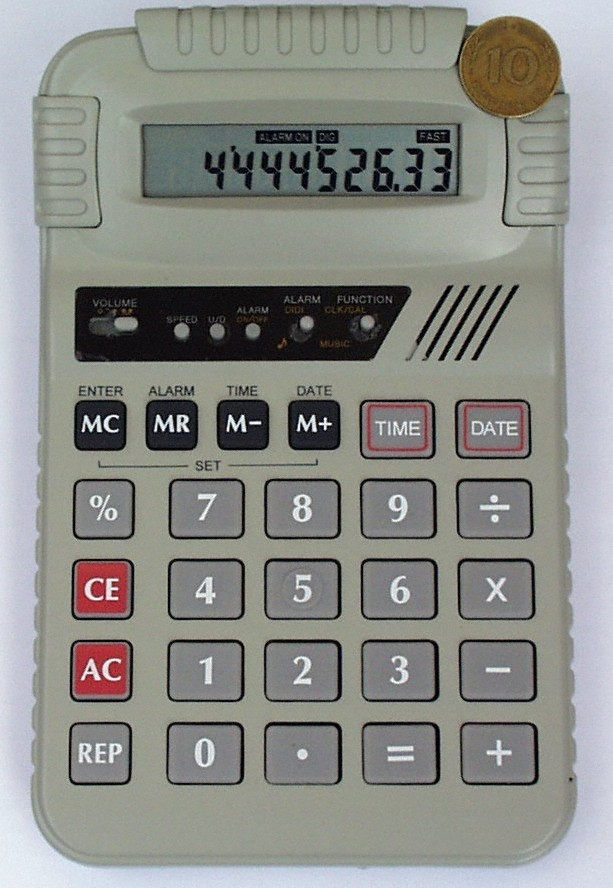
\includegraphics[width=.4\textwidth]{taschenrechner.jpg}
\end{center}
\h{Jetzt sogar mit Glückspfenning!}

Dies ist ein \url{http://mitschriebwiki.nomeata.de/}-Projekt. Mitgewirkt haben: Joachim Breitner, Wenzel Jakob, Martin Kiefel, Lucas Lürich und Jennifer Tesch.
\end{document}
